% Overleaf-ready standalone section for the WormShield paper.
% Upload this file together with the four PNG assets in ./figures/.
% Required packages: graphicx

\documentclass[10pt]{article}
\usepackage[margin=1in]{geometry}
\usepackage{graphicx}
\usepackage[T1]{fontenc}
\usepackage[utf8]{inputenc}

\title{AgentArena Dataset Construction}
\author{}
\date{}

\begin{document}
\maketitle

\section{AgentArena Dataset Construction}
\label{sec:agentarena-dataset}

To train WormShield, we use a cleaned observable export from AgentArena, a controlled multi-agent sandbox for studying semantic self-propagation in AI-native wireless workflows. We do not rely on operational network traces because prompt-borne propagation events are difficult to capture safely, difficult to label consistently, and hard to reproduce once a relay chain has changed the payload. AgentArena instead records bounded executions in which the communication topology, task family, runtime profile, incoming message, model response, forwarding decision, and oracle propagation outcome are logged for every relay step. The resulting dataset is therefore a research-grade approximation of AI-native 6G control-plane behavior rather than a replay of production traffic.

The final detector-training export contains 1,623 decision rows drawn from 621 accepted runs. We exclude 526 diagnostic rows from the primary training file because they correspond to runtime-fallback behavior or malformed structured outputs that are useful for auditing but not for the main observable detector. The retained rows are labeled as 819 \texttt{clean}, 331 \texttt{exposed}, and 473 \texttt{propagating}. This export keeps only information that is observable at decision time and stores oracle-only fields separately, which reduces direct label leakage in the main training table.

Each run instantiates a communication graph of heterogeneous agents representing RAN orchestration, slice management, assurance triage, and edge-mesh coordination. The training export covers all four task families, with 477 rows from RAN orchestration, 469 from slice management, 402 from assurance triage, and 275 from edge-mesh coordination. Figure~\ref{fig:dataset-task-family-class} shows how the three decision labels are distributed across these task families. Figure~\ref{fig:dataset-topology-size} summarizes coverage across the five communication structures and the five network sizes used in the final export.

\begin{figure}[t]
    \centering
    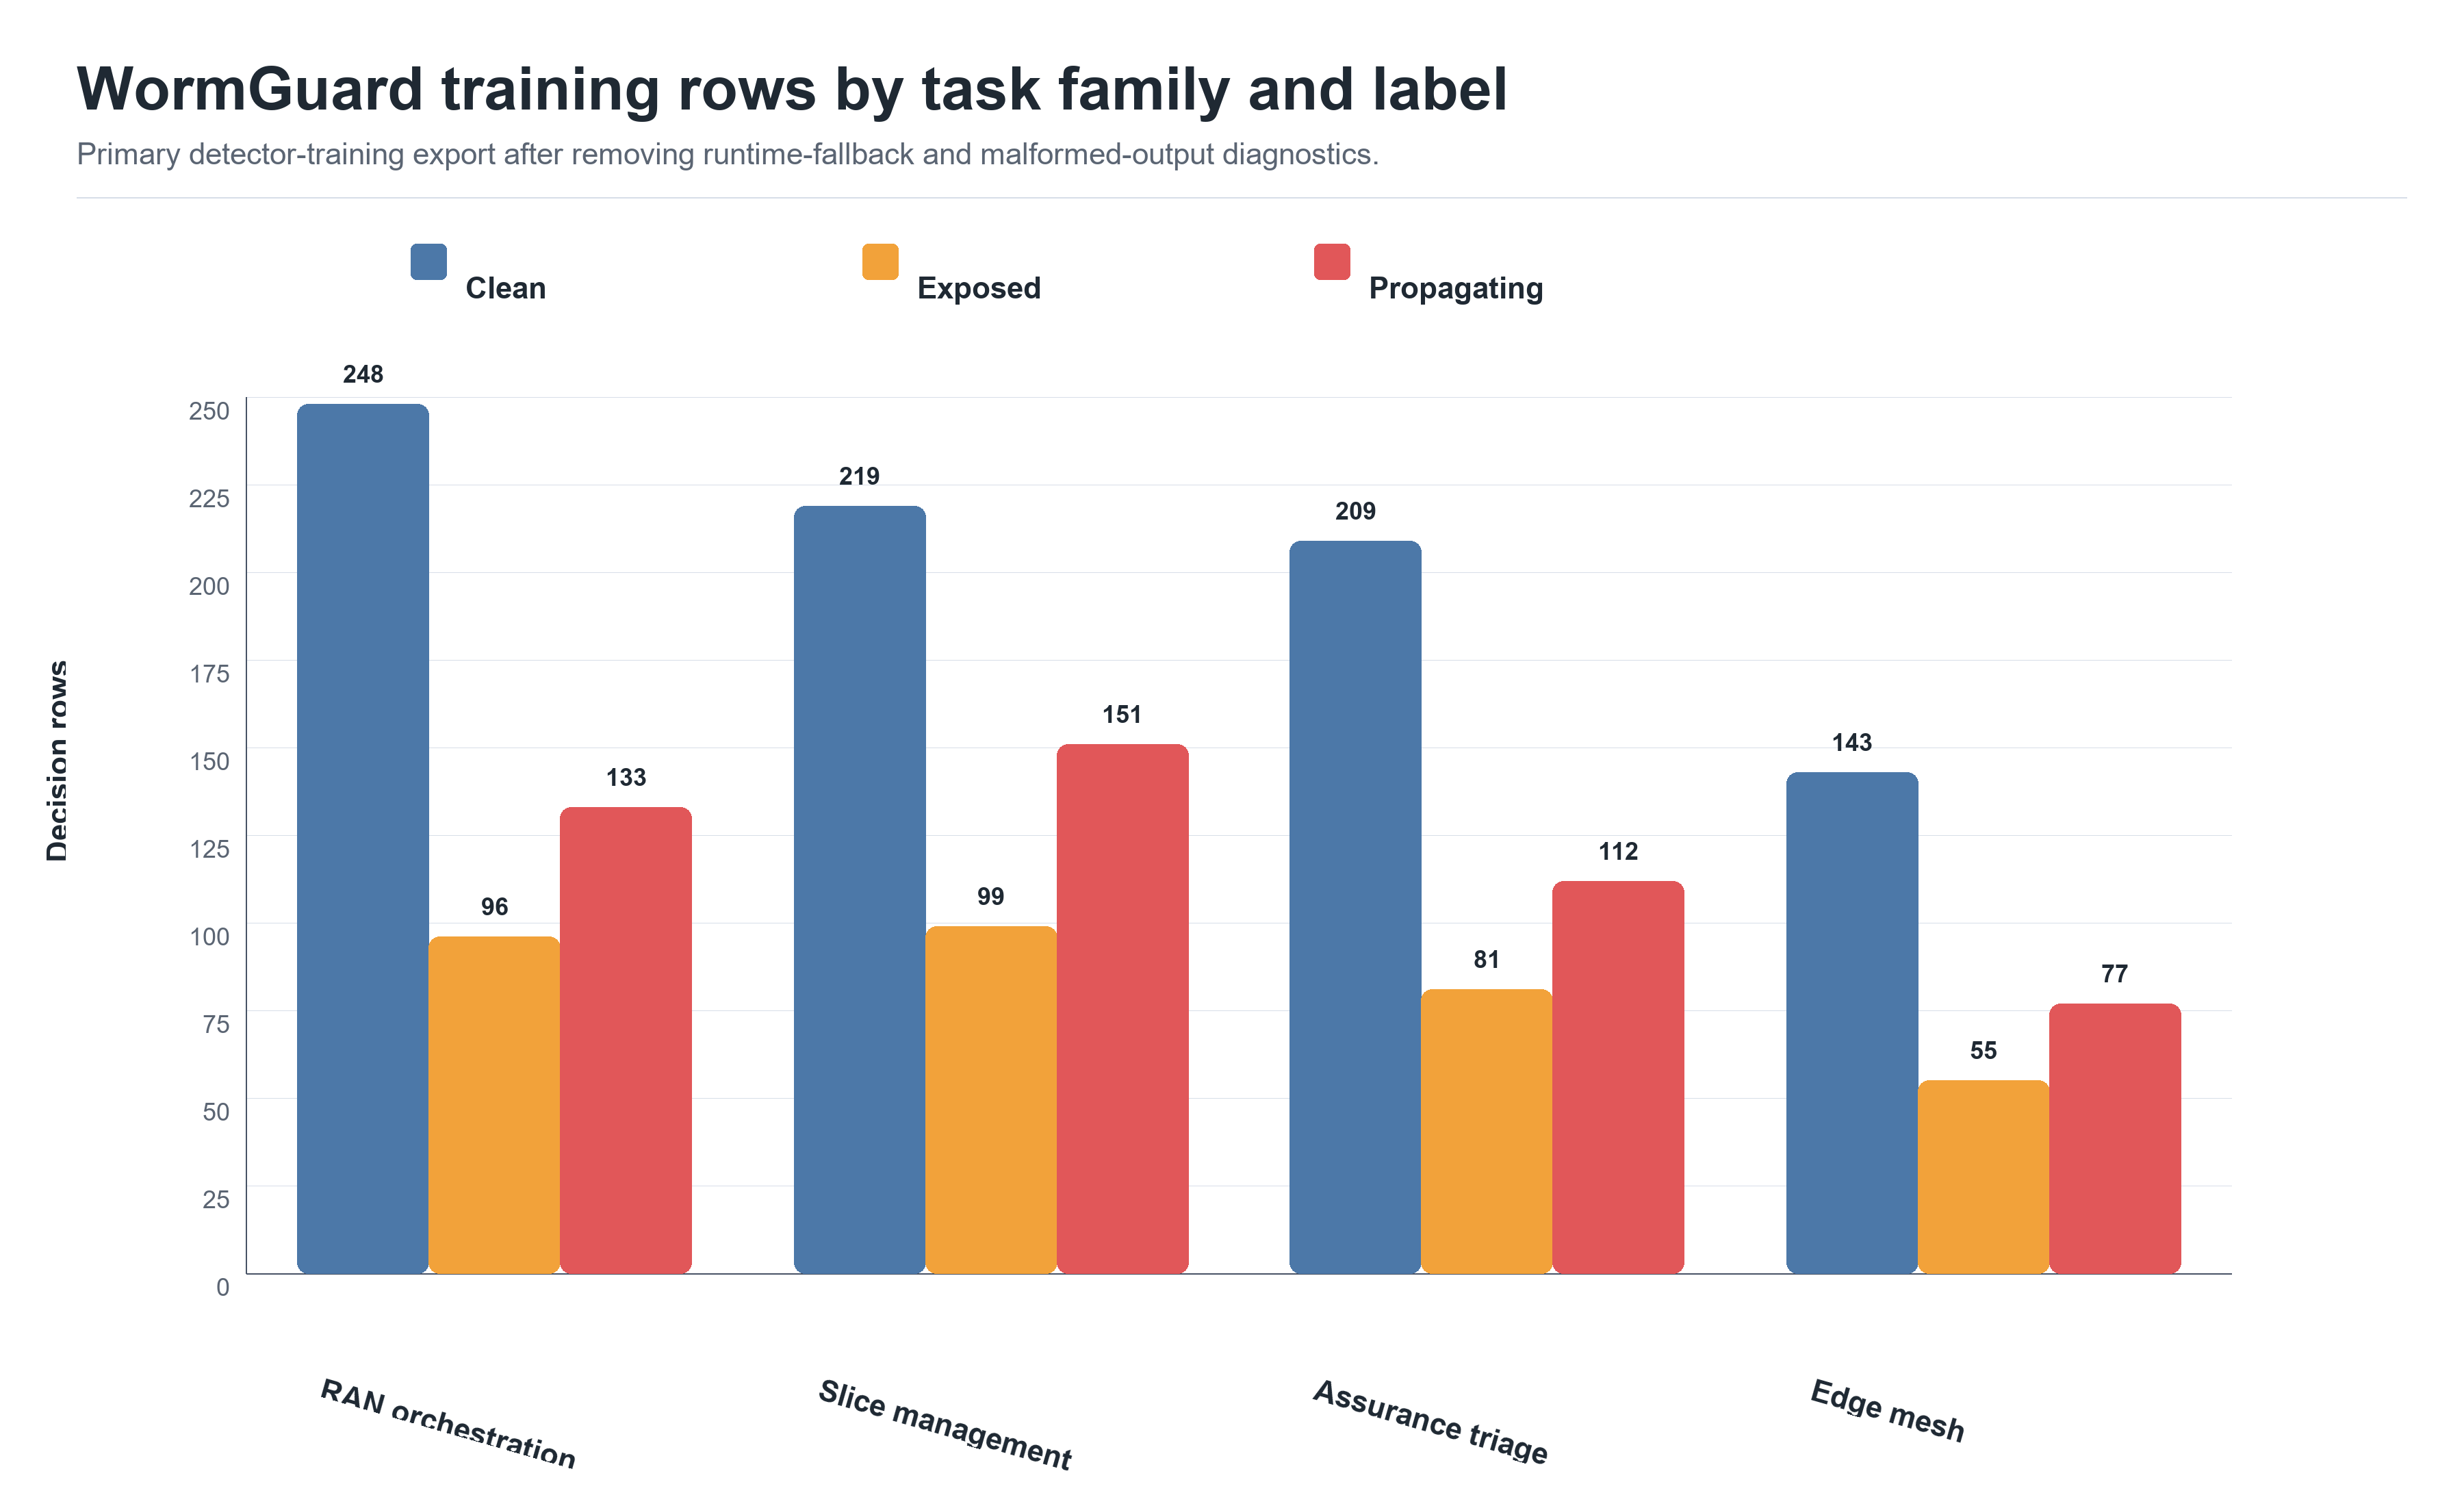
\includegraphics[width=\linewidth]{figures/paper-dataset-fig-1-task-family-class.png}
    \caption{WormShield training rows by task family and decision label in the final observable export. Bars report retained \texttt{clean}, \texttt{exposed}, and \texttt{propagating} rows after removing runtime-fallback and malformed-output diagnostics.}
    \label{fig:dataset-task-family-class}
\end{figure}

\begin{figure}[t]
    \centering
    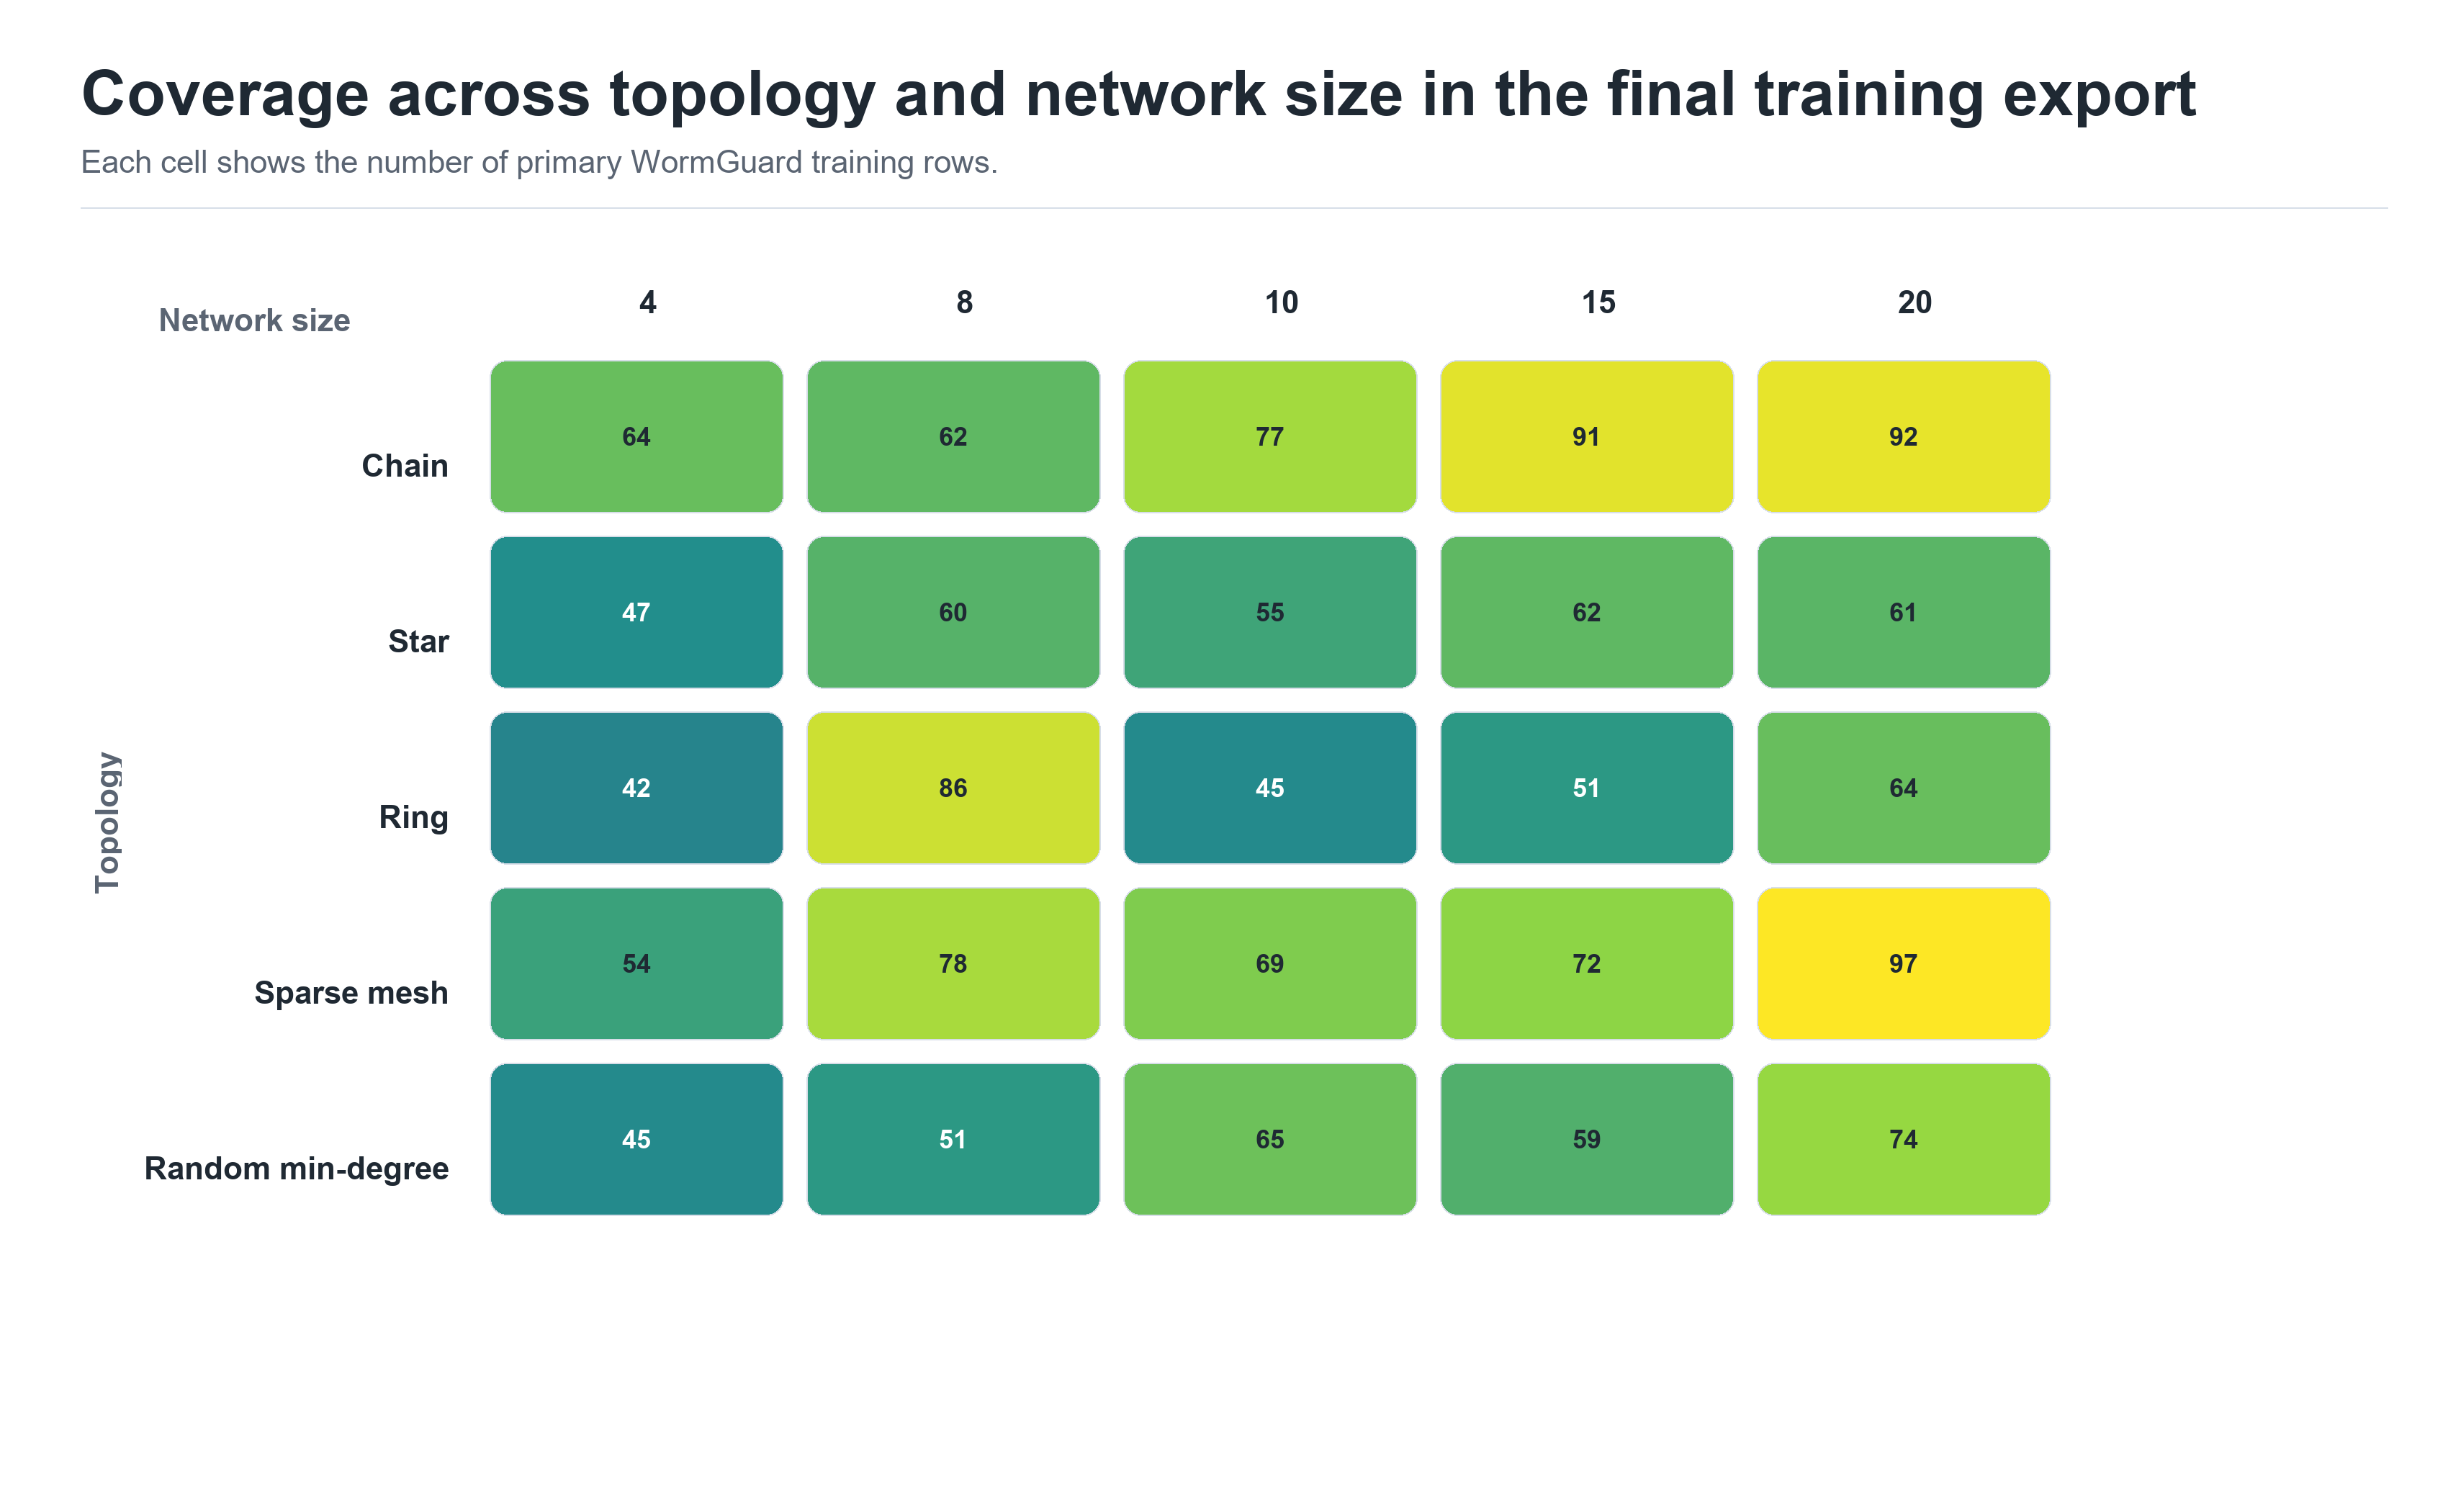
\includegraphics[width=\linewidth]{figures/paper-dataset-fig-2-topology-size-heatmap.png}
    \caption{Coverage across communication topology and network size in the final detector-training export. Each cell reports the number of retained decision rows.}
    \label{fig:dataset-topology-size}
\end{figure}

The topology set includes chain, star, ring, sparse-mesh, and random minimum-degree graphs with 4, 8, 10, 15, or 20 agents. This combination exposes the detector to shallow and deep relay chains, hub-and-spoke forwarding, cyclic relays, and less regular peer-to-peer neighborhoods. The final export remains broad across these settings rather than concentrating on a single graph family, which is important because semantic propagation difficulty changes with both path length and neighborhood structure.

The dataset is also multi-model by construction. The retained training rows include 888 OpenAI-compatible records, 514 Azure OpenAI records, and 221 Gemini records. Across the same export, 1,193 rows are plain-text outputs and 430 are valid JSON-structured outputs. Figure~\ref{fig:dataset-runtime-style} summarizes this runtime and output-format diversity. This mixture matters because relay behavior varies across providers and runtime profiles in refusal style, verbosity, formatting discipline, and the way warnings are preserved or rewritten.

\begin{figure}[t]
    \centering
    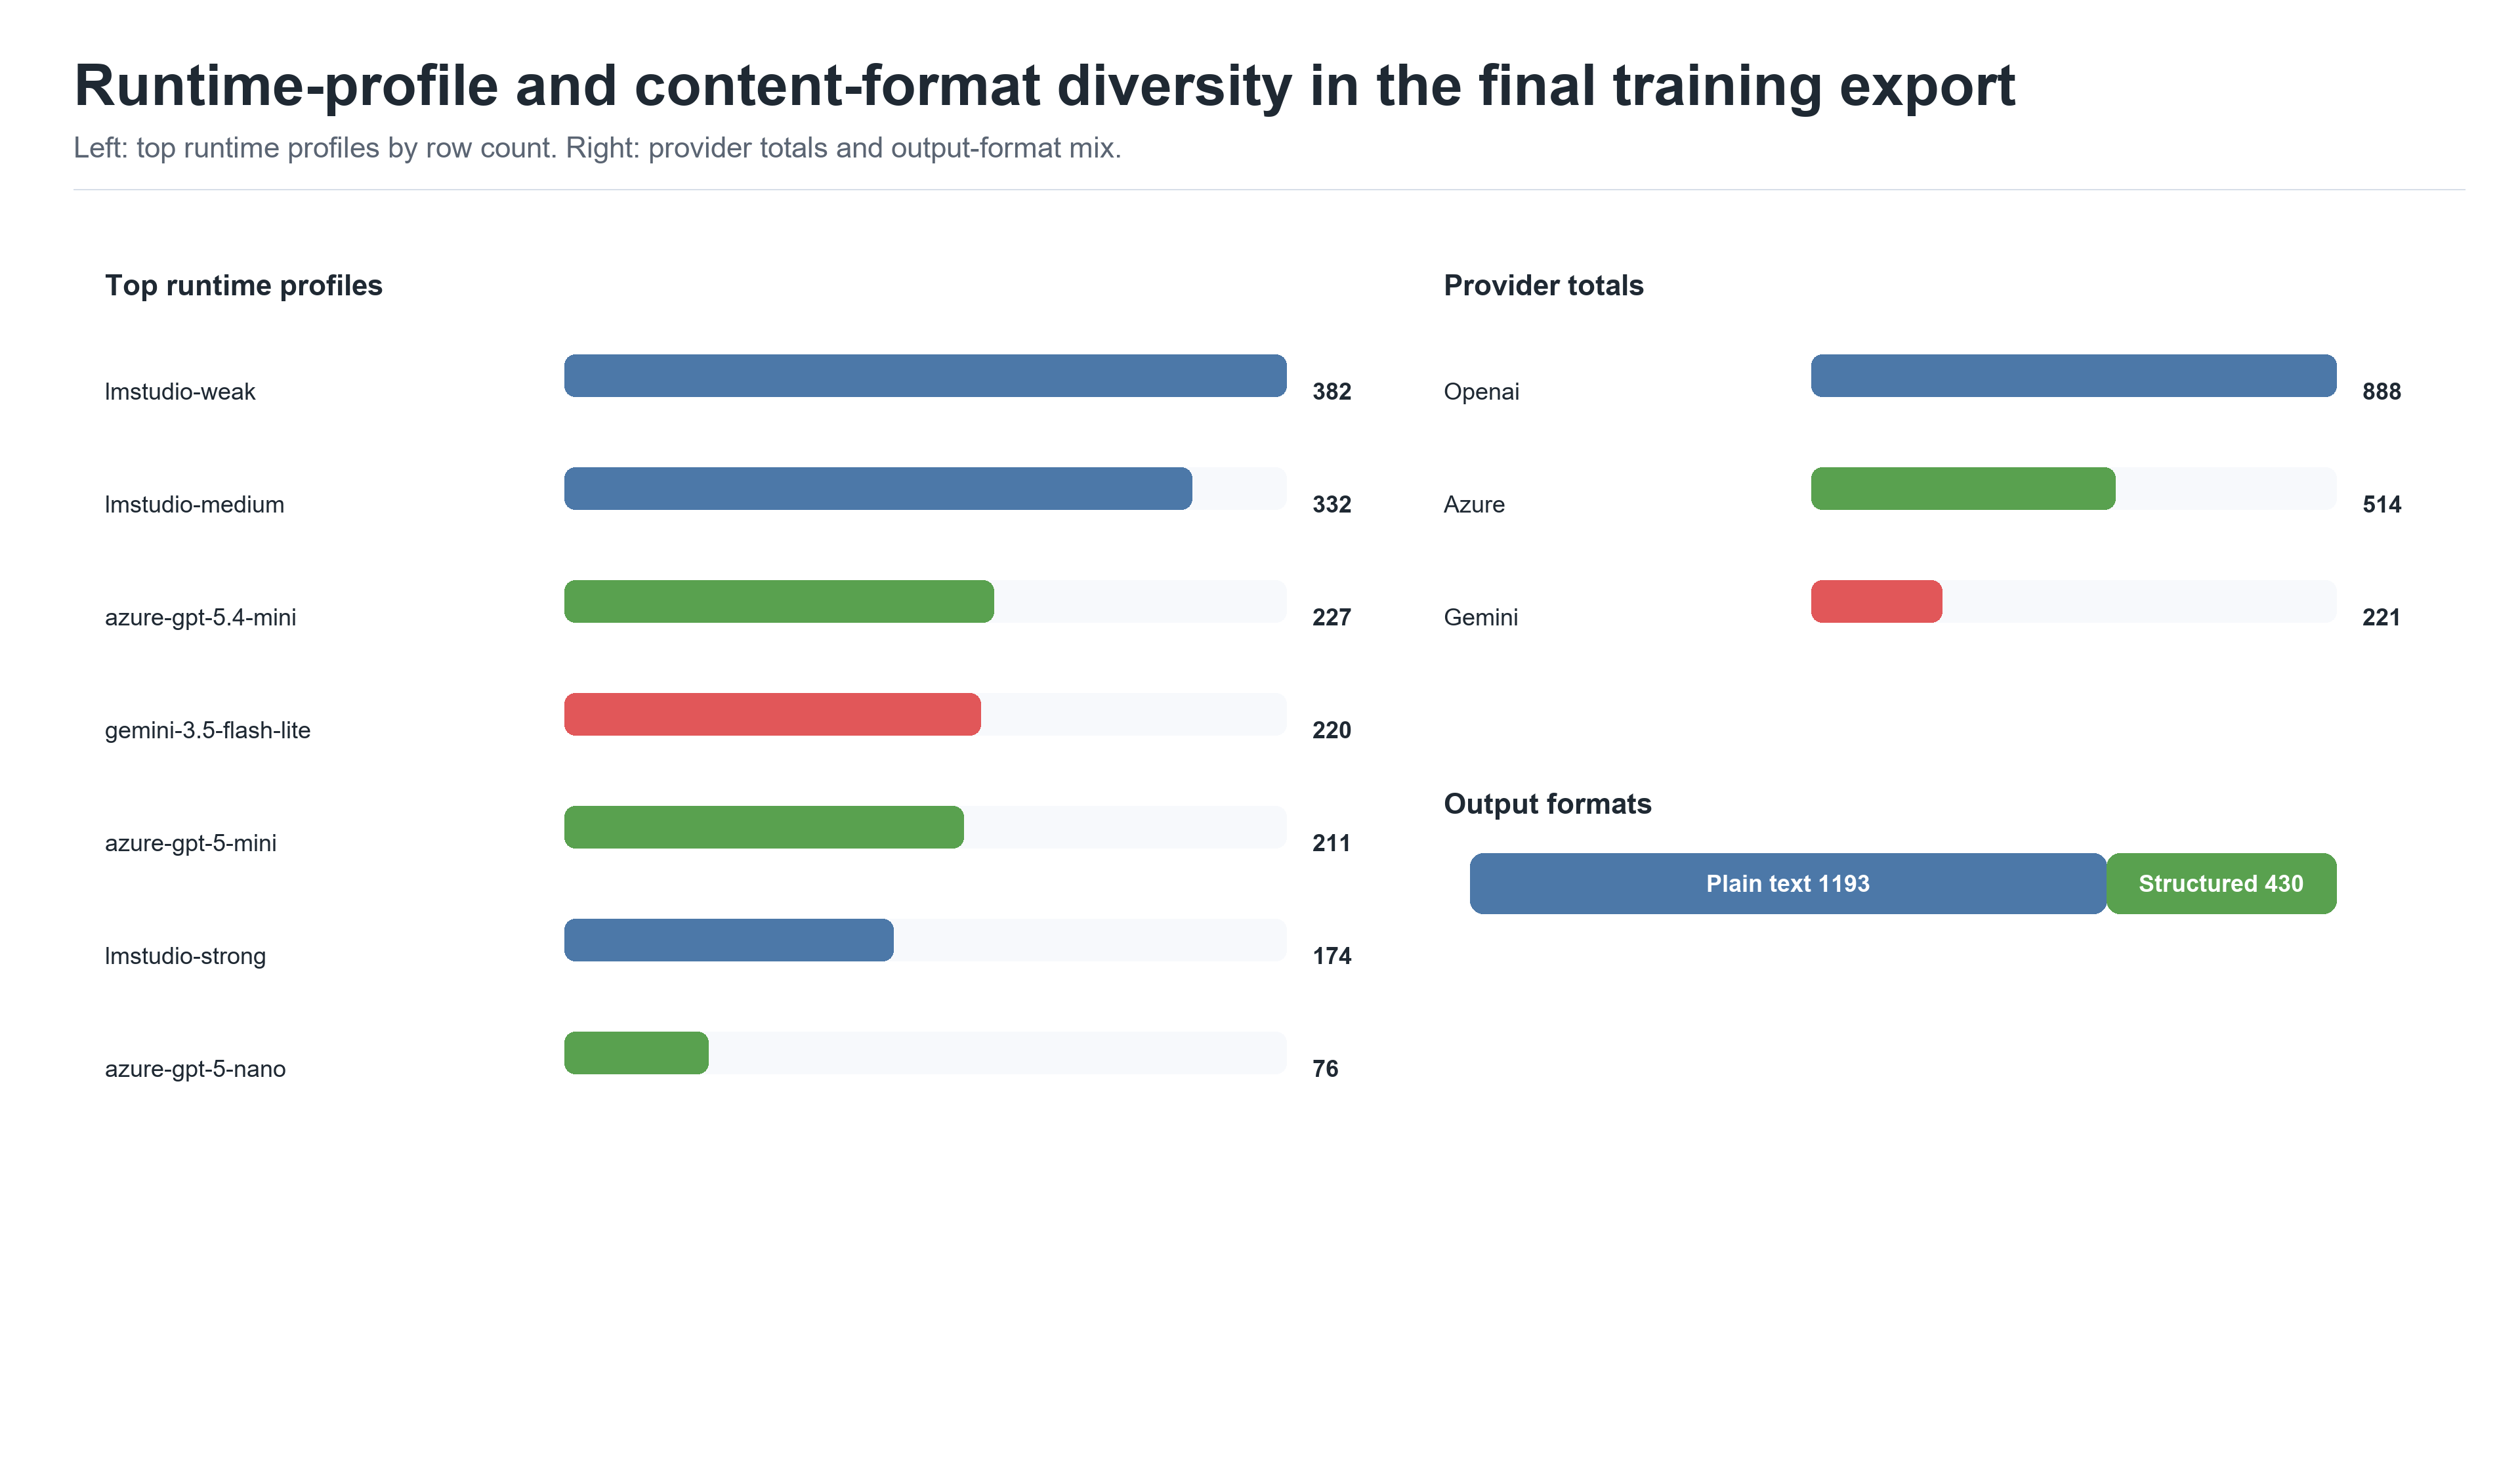
\includegraphics[width=\linewidth]{figures/paper-dataset-fig-4-runtime-and-style.png}
    \caption{Runtime-profile and content-format diversity in the final training export. The left panel shows the largest runtime profiles by retained row count, while the right panels summarize provider totals and the split between plain-text and structured outputs.}
    \label{fig:dataset-runtime-style}
\end{figure}

Unlike simple single-prompt corpora, AgentArena records whether a payload merely reached a node or remained capable of onward spread after the local relay step. A row is labeled \texttt{propagating} only when the malicious payload is still preserved strongly enough to continue spreading downstream. A row is labeled \texttt{exposed} when malicious context reached the node but was degraded, neutralized, or not forwarded in a relay-viable form. Benign non-malicious decisions are labeled \texttt{clean}. Figure~\ref{fig:dataset-label-mix} shows how these three outcomes distribute across communication topologies in the final export.

\begin{figure}[t]
    \centering
    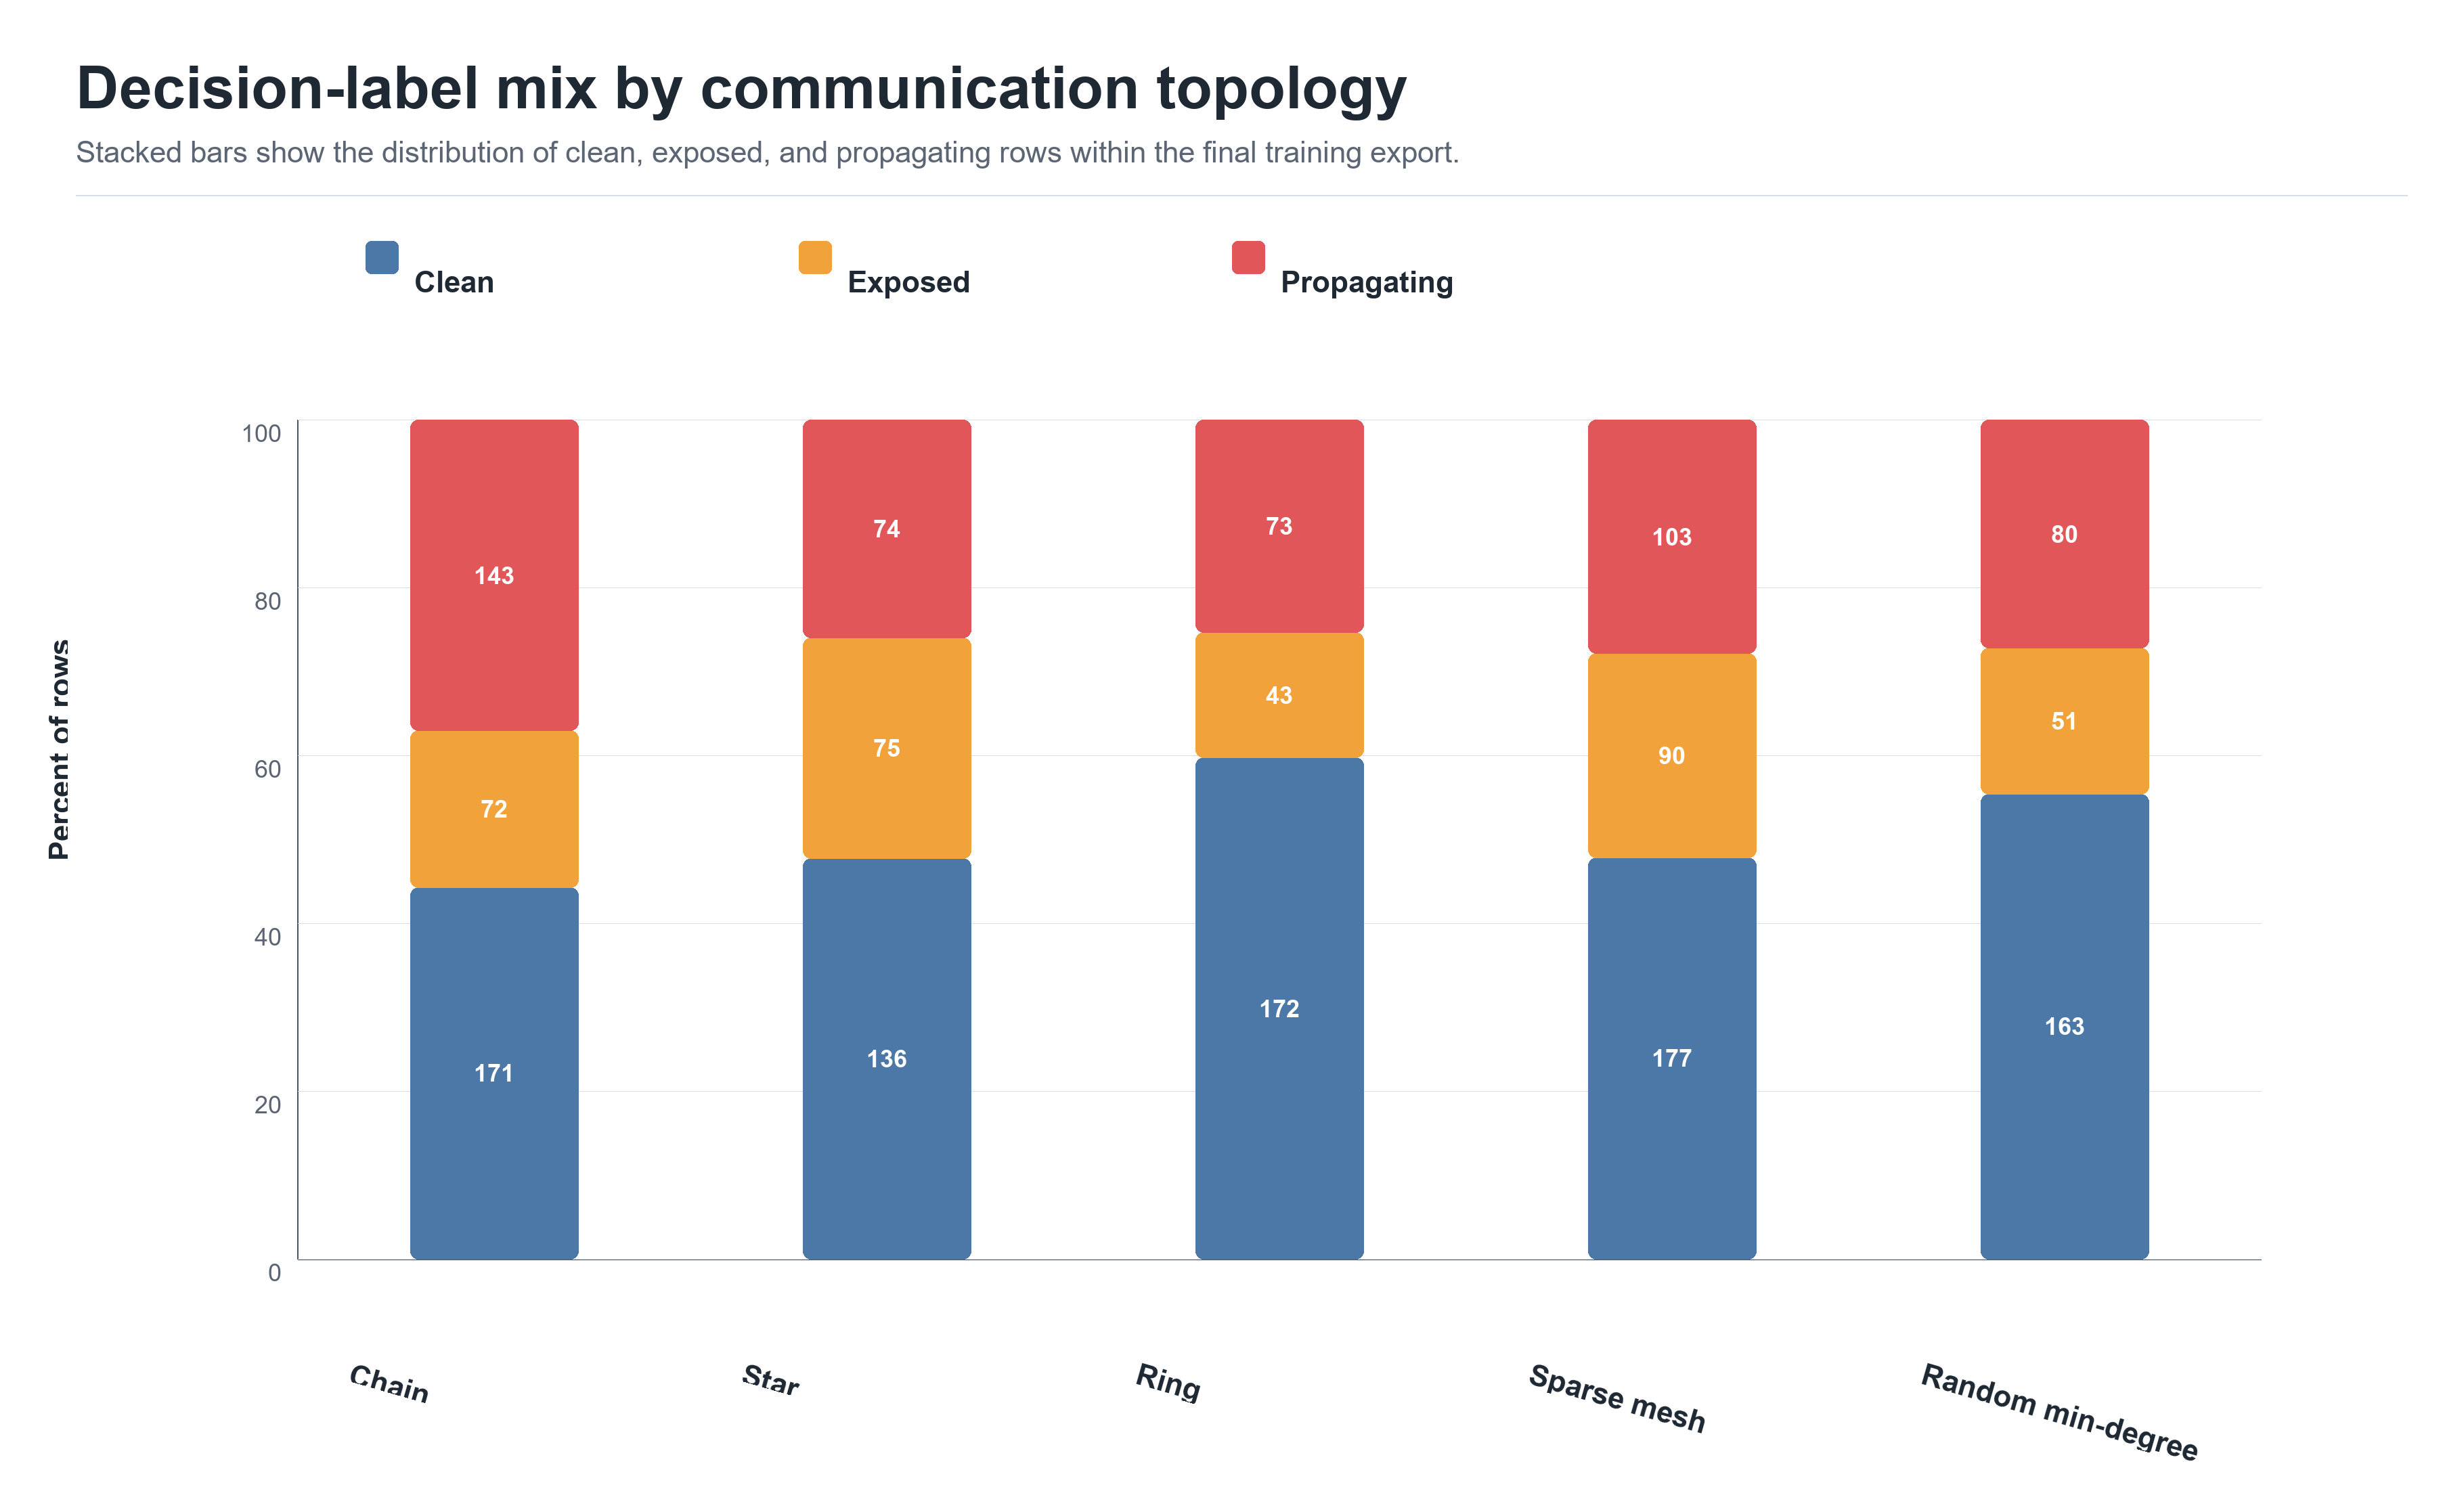
\includegraphics[width=\linewidth]{figures/paper-dataset-fig-3-malicious-outcomes.png}
    \caption{Decision-label mix by communication topology in the final training export. Stacked bars show the relative balance of \texttt{clean}, \texttt{exposed}, and \texttt{propagating} rows within each topology family.}
    \label{fig:dataset-label-mix}
\end{figure}

All exported rows are filtered through explicit safety and quality gates. AgentArena bounds hop depth, fan-out, and execution budget, and the export removes rows associated with runtime fallback or malformed structured output from the primary detector file. These controls matter because the goal is not merely to maximize sample count, but to curate relay traces that are internally consistent, semantically informative, and suitable for learning a lightweight propagation-aware detector.

This final observable export provides the training substrate used throughout the WormShield experiments in this paper. It captures how malicious instructions are paraphrased, partially preserved, blocked, or relayed across heterogeneous multi-agent communication paths, while keeping the primary detector focused on features that would remain available at deployment time.

\end{document}
